\section{Local Search}
	On ne s'occupe pas du path dans cette partie, notre but est d'avoir le Goal
	\begin{itemize}
		\item Utilise peut de mémoire
		\item Peut trouver des solution dans une infinité de recherche
		\item Trouve des solutions raisonnable (pas optimal)
	\end{itemize}
	
	On améliore itérativement la solution actuelle. La prochaine solution est dans le voisinage (\textbf{neighborhood}) de la solution actuelle.
	
	\subsection{Optimisation probleme}
		On a une \textbf{Fonction objetive} que on peut maximiser ou minimiser. On veut trouver le Max/Min Global (par ex: distance, nb de queens sur le plateau ...). Le probleme sont les Max/Min locaux et on peut rester coincé dessus.
		
		\begin{figure}[htp]
			\centering
			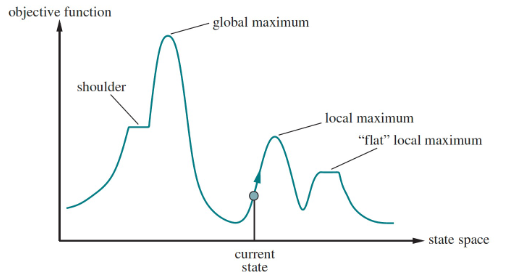
\includegraphics[width=0.5\textwidth]{img/LocalOptiProbleme.png}
		\end{figure}
	\subsection{Neighbourhood}
	
		\textbf{Size}		
	
		Si on décide de choisir un grand \textit{voisinage}, on va avoir des path plus petit pour la solution, mais on va avoir besoin de plus de temps pour parcourir toutes les possibilités. Ils faut trouver un juste milieu entre longueur des paths et temps d'explorations
		
		\textbf{Connectivity}
		
		Pour chaque solution, il y a un path a une solutions optimal. Cela a 2 avantages :
		\begin{itemize}
			\item Pas besoin de recommencer la stratégie (on ne bloque jamais)
			\item Nécessaire pour la propriété de convergence
		\end{itemize}

		\textbf{Contraintes}
		
		Il y a 2 approche possible pour combiner faisabilité avec requièrement optimal
		\begin{itemize}
			 \item Approche 1
			 \begin{itemize}
			 	\item Maintenir la faisabilité à tout moment
			 	\item Explorer seulement les solutions faisable 
			 \end{itemize}
			 \item Approche 2
			 \begin{itemize}
			 	\item Ne pas maintenir la faisabilité à tout moment ;
assouplir un sous-ensemble de contraintes
				\item Explorer un plus grand \textit{Search Space}
				\item Conduire a chercher a des solutions faisable et de qualités
			 \end{itemize}
		\end{itemize}
		
		Un exemple car c'est un peu trop théorique : Graph partitioning
		S
		\begin{figure}[htp]
			\centering
			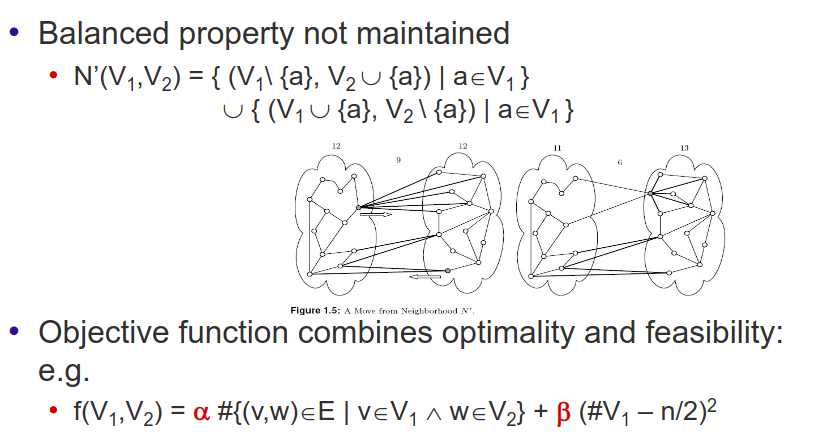
\includegraphics[width=0.7\textwidth]{img/exempleGraphPartionning.png}
		\end{figure}
	\subsection{Heuristic et Metaheuristics}
		\textbf{Heuristics}
		Se concentre sur choisir la prochaine solutions et conduire la recherche avec des optimum local basé sur l'information locale (solutions actuelle et le neighbourhood). utilise peu de mémoire
		
		\textbf{Metaheuristics}
		Tente d'échapper les optimum locaux pour trouver le global optimum basé sur la collecte d'information avec les exécutions faites avants. Prend plus de mémoire car learning derrière.
		
		\textbf{Systematic heuristics}
		Exploration (partiellement possible) du voisinage  pour déterminer solution suivante.
		
	\subsection{Hill Climb Algo}
		\begin{figure}[htp]
			\centering
			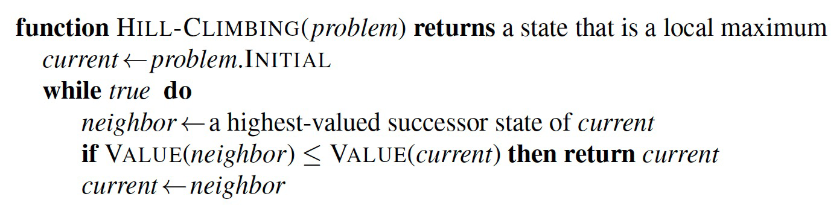
\includegraphics[width=0.7\textwidth]{img/CodeHillClimb.png}
		\end{figure}
		On choisi un state de départ, et on avance dans la direction des valeurs qui augmentes et on stop l'itération quand on ne peut plus aller plus loins. Cette algo va rapidement a la meilleure  solutions mais a plusieurs probleme :
		\begin{itemize}
			\item S'arrête si c'est un Max/Min local
			\item Si on a un plateau, l'algo se stop (on peut mettre un limite d'itération si on tombe la dessus)
			\item Si on a une séquence de Max/Min locaux alors on a du mal a naviguer
		\end{itemize}
		
		Hill climb dépend énormément de la forme du state space et vu que il ne fera jamais de down-hill, si il tombe sur un maxLocal il reste bloqué
		
		\begin{figure}[htp]
			\centering
			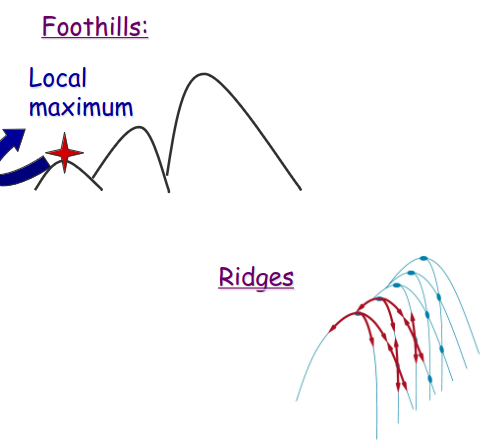
\includegraphics[width=0.6\textwidth]{img/ProblemHillClimb.png}
		\end{figure}			
		
	\subsubsection{Varaintes}
		Il existe plusieures variantes:
		\begin{itemize}
			\item \textbf{Stochastic hill climbing} : Choisis en mode random parmis les mouvements qui monte
			\item \textbf{First-choice hill climbing} : On choisi le premier bon successeur que on trouve, pratique si le nombre de successeur est large
			\item \textbf{Random restart} : On commence de plusieurs points random
		\end{itemize}
	
	\subsection{Random Walk}
		On sélectionne en mode random un élément du neighbourhood et on décide si on doit l'accepter comme la prochaine solution. Il y a plusieur approche possible :
		\begin{itemize}
			\item Amélioration aléatoire
			\item Heuristique de Metropolis : accepter de dégrader la solution
		\end{itemize}
		
	\subsection{Simulated annealing}
		Algo qui combine Hill climb, un scheduler et un metropolis step.
		\begin{itemize}
			\item Toujour avance en montant (uphill) si possible
			\item Parfois aller en descendant (downhill) 
		\end{itemize}
		
		On commence avec beaucoup de random et on reduit graduellement l'intensité du random dans l'algo (Annalogie avec la métalirgue qui chauffe du fer et le laisse refroidir lentement)
		
		Opérations :
		\begin{enumerate}
			\item Toujours aller uphill si possible
			\item parfois (random) aller downhill (quand la témpérature est haute faut laisser redescendre)
			\item C'est assurée d'etre optimal si réduction lente.
		\end{enumerate}
				
	\subsection{Local Beam Search}
		Mélange de hillclimb et annealing en gardant un seul state en mémoire. L'idée est de :
		\begin{enumerate}
			\item garder $k$ states en mémoire
			\item chaque step, générer tous les successeur des $k$ states
			\item On stop si un state est un goal
			\item Sinon, on sélectionne les $k$ meilleur successeurs de la liste complète de tous les successeurs
		\end{enumerate}
		
		L'algo souffre d'un manque de diversité car les states converges rapidement vers la  régions
		
	\subsection{Genetic Algorithms (GAs)}
		Basée sur la théorie de l'évolution (woké en panique). On commence avec $k$ supposition de début (populations), chaque individus  de la population a un string de longueur fixe qui représente son gêne. On produit la prochaine génération en \textbf{reproduisant} les individus de la populations en ajoutants quelque random mutations. Chaque individus possèdes un score de fitness
		
		\begin{figure}[H]
			\centering
			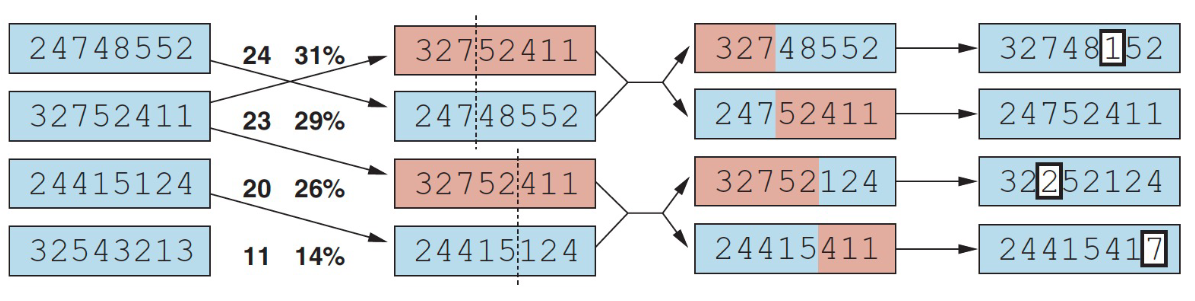
\includegraphics[width=0.7\textwidth]{img/GA}
		\end{figure}
	
		Exemple 8-queens:
		\begin{figure}[htp]
			\centering
			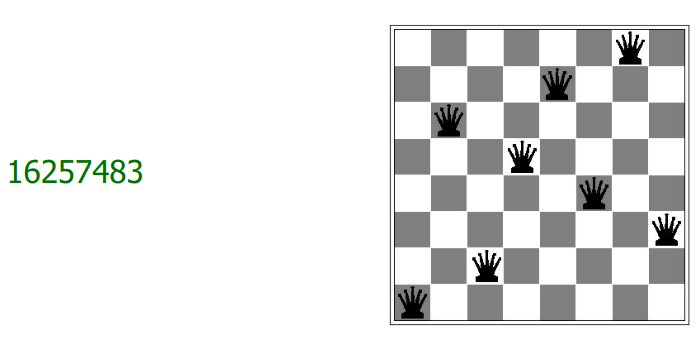
\includegraphics[width=0.5\textwidth]{img/8QueenGA1.png}
			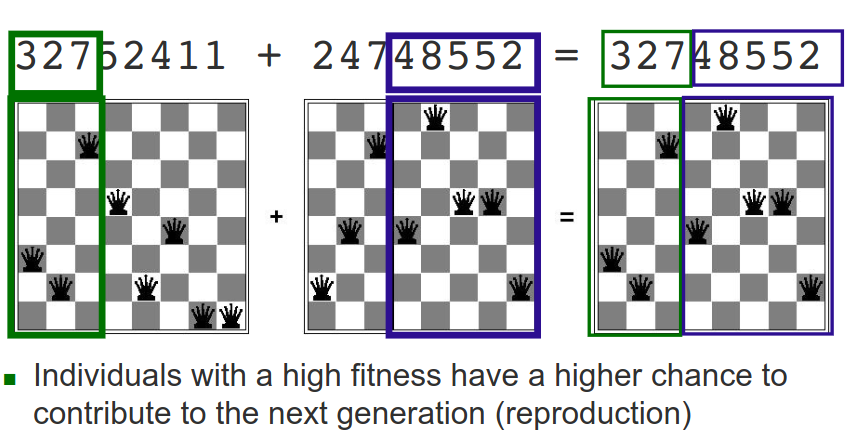
\includegraphics[width=0.7\textwidth]{img/8QueenGA2.png}
		\end{figure}
		
		Les mutations randoms peuvent amener a un bonne situation et permet d'explorer de nouvelle partie du search space
		
		\begin{figure}[htp]
			\centering
			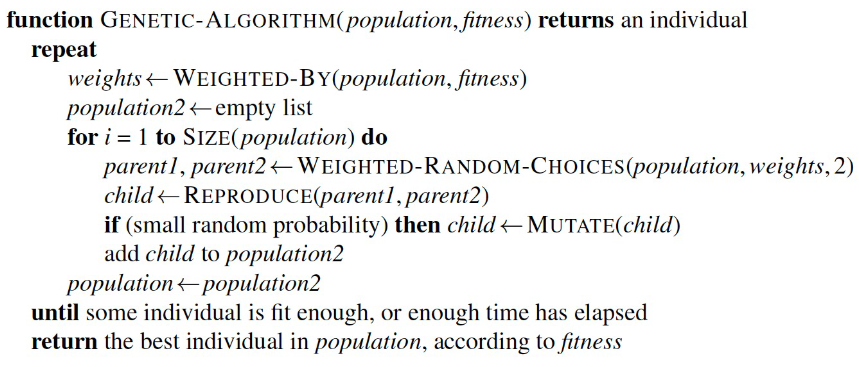
\includegraphics[width=0.7\textwidth]{img/AlgoGA1.png}
			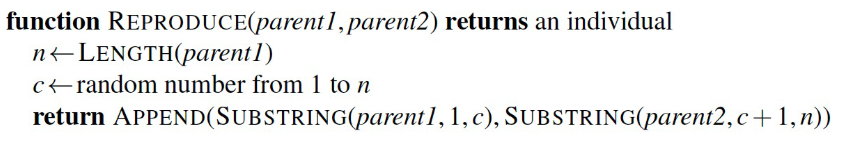
\includegraphics[width=0.7\textwidth]{img/AlgoGA2.png}
		\end{figure}
		
		un probleme avec cet algo est que le crossover est pas applicable a tous les problèmes.
		
	\subsection{Tabu search Metaheuristics}
		
		Sélectionne le meilleur voisin \textbf{qui a pas encore été visité}. Un problème est que c'est difficile de garder la trace de tous les nodes déja visités. Un solutions est de garder en mémoire un suffix de la séquence de node visité.
		
	\subsection{Intensification vs. Diversification}
		\begin{tabular}{|l|p{0.45\textwidth}|p{0.45\textwidth}|}
			\hline
			& Intensification & Diversification\\
			\hline
			\textbf{Goal} & Accroître la recherche dans les domaines prometteurs & Explorer de nouveaux endroit\\
			\hline
			\textbf{Risk} & Convergence prématurée (Max/Min Local) & Convergence vers l'optimal peut prendre du temps\\
			\hline
			\textbf{Mean} & Favorise les bonne solutions & Choix probabiliste des solutions\\
			\hline
			
		\end{tabular}
		
	\subsection{Other Local Search}
		\begin{itemize}
			\item \textbf{Variable Neighborhood Search}
			\item \textbf{Guided Local Search}
			\item \textbf{Adaptive Local Search}
			\item \textbf{Ant Colony Optimization}
			\item \textbf{Statistic Local Search} \footnote{voir slides}
		\end{itemize}
		
	\newpage